% ======================================================================
% main.tex -- SPEC 0055 insight-first expert deck (16:9 TUD).
%
% Build:          cd presentation/beamer && make
%
% Insight-first talk for Trackastra / ML lab experts. Figures are reused
% read-only from ../../report-shorten/figs/; no tutorial content and no
% generated talk figures. Slide content lives in slides/*.tex.
% The TUD theme, assets, and fonts are read-only.
% ======================================================================
\documentclass[aspectratio=169]{beamer}
\usetheme{TUD}

\usepackage{hyperref}
\usepackage{array}
\usepackage{booktabs}
\usepackage{amsmath}
\usepackage{tikz}
\usetikzlibrary{positioning,arrows.meta,calc,fit,backgrounds}
\usepackage[backend=biber,style=numeric,sorting=none]{biblatex}
\addbibresource{references.bib}

\graphicspath{{assets/}{../../report-shorten/figs/}}

\title{Efficient sparse attention and self-supervised learned features for transformer-based cell tracking}
\author{Leonard Starke}
\date{28.10.2026}

\renewcommand\TudFooterText{Efficient sparse attention \& self-supervised features for cell tracking \textbullet{} Leonard Starke}

\begin{document}

% ======================================================================
% 00-opening.tex -- SPEC 0055, frames 1-3.
%
% Insight-first opening for Trackastra / ML lab experts. Three frames:
% title; the questions and the evidence standard; five unexpected findings.
% The proposal map, the "bar", the exploration table, and the "three claims"
% slide are deliberately removed. No tutorial exposition.
%
% Shared lane definitions:
%   - palette: talkred, talkorange, talkteal, talkgray, talklight,
%     talkblue, talkgreen
%   - \talksectiondivider{<large title>}{<one-line subtitle>}
% ======================================================================

% ----------------------------------------------------------------------
% Shared palette (used by all slide lanes).
% ----------------------------------------------------------------------
\definecolor{talkred}{HTML}{C00000}
\definecolor{talkorange}{HTML}{D97706}
\definecolor{talkteal}{HTML}{00756F}
\definecolor{talkgray}{HTML}{5A5A5A}
\definecolor{talklight}{HTML}{EEF2F6}
\definecolor{talkblue}{HTML}{00008C}
\definecolor{talkgreen}{HTML}{1F7A5C}

% ----------------------------------------------------------------------
% \scite{<keys>} -- small inline citation.
% Keeps the reference marker a superscript so citations stay in the text
% flow; the deck does not use bottom captions or footnotes for sources.
% ----------------------------------------------------------------------
\newcommand{\scite}[1]{\textsuperscript{\cite{#1}}}

% ----------------------------------------------------------------------
% \talksectiondivider{<large title>}{<one-line subtitle>}
% One centered divider frame with vertical fill above and below. Section
% lanes call this at top level; #1 uses the TUD slide-title face.
% ----------------------------------------------------------------------
\newcommand{\talksectiondivider}[2]{%
  \begin{frame}
    \vfill
    \centering
    {\TudSlideTitleFont\fontsize{6.5mm}{7.4mm}\selectfont
      \textcolor{tudblue}{#1}\par}
    \vspace{3mm}
    {\normalsize\textcolor{talkgray}{#2}\par}
    \vfill
  \end{frame}
}

% ----------------------------------------------------------------------
% \talktitle{<title text>}
% Wrap slide titles in a 0.90-textwidth parbox so long titles wrap inside
% the frame instead of running past the right edge. \smash gives the title
% zero height, so a wrapped multi-line title does not shift the body into
% the title band; the theme still draws the title overlay and footer.
% ----------------------------------------------------------------------
\newcommand{\talktitle}[1]{\frametitle{\smash{\parbox[t]{0.90\textwidth}{\raggedright\fontsize{4.8mm}{5.3mm}\selectfont #1}}}}

% ----------------------------------------------------------------------
% Frame 1 -- title page.
% ----------------------------------------------------------------------
\begin{frame}[plain]
  \TudTitlePage{Efficient sparse attention and\\self-supervised learned features for\\transformer-based cell tracking}{Leonard Starke \\ Research Assignment \\ 28.10.2026}
\end{frame}

% ----------------------------------------------------------------------
% Frame 2 -- questions and the evidence standard.
% Claim: each question has a pre-committed test, not a post-hoc narrative.
% ----------------------------------------------------------------------
\begin{frame}
  \talktitle{What we set out to learn}
  \centering
  \hyphenpenalty=10000
  \exhyphenpenalty=10000
  \small
  \renewcommand{\arraystretch}{1.45}
  \begin{tabular}{@{}>{\raggedright\arraybackslash}p{61mm}>{\raggedright\arraybackslash}p{64mm}@{}}
    \toprule
    {\raggedright\textbf{Question}} & {\raggedright\textbf{What would count as evidence}}\\
    \midrule
    {\raggedright Where does the cost of the cutoff mask actually live?} &
    {\raggedright Kernel-verified dispatch; production batch $B{=}64$.}\\
    {\raggedright Can a warp manufacture association labels without annotations?} &
    {\raggedright Held-out \texttt{trpL}; pre-registered rule; compute-matched control.}\\
    {\raggedright Which signal carries association: position and geometry, or learned features?} &
    {\raggedright Coordinates-only candidates; frame-CV and LOCO.}\\
    \bottomrule
  \end{tabular}
  \vspace{4mm}

  {\footnotesize The talk reports what changed our mind, not what the proposal hoped.\par}
\end{frame}

% ----------------------------------------------------------------------
% Frame 3 -- five unexpected findings.
% Claim: the talk's payload is these five results, each backed by a measured
% artifact; the rest of the deck supplies the evidence and the bounds.
% ----------------------------------------------------------------------
\begin{frame}
  \talktitle{Five things we did not expect}
  \centering
  \hyphenpenalty=10000
  \exhyphenpenalty=10000
  \small
  \renewcommand{\arraystretch}{1.35}
  \begin{tabular}{@{}p{6mm}>{\raggedright\arraybackslash}p{103mm}p{17mm}@{}}
    \toprule
    \textbf{\#} & {\raggedright\textbf{Finding}} & \textbf{Section}\\
    \midrule
    1 & The mask already reaches a fused cuDNN kernel; the mask itself is the cost. & \S4.1\\
    2 & Removing the cutoff costs accuracy in 12/12 fold--seed cells. & \S4.1\\
    3 & Attention is 10.05\% of the step; the norm chain is 38.7\%. & \S4.1\\
    4 & The warp pretext collapses to all-negative for a structural reason. & \S4.2\\
    5 & Position and geometry beat learned features by 0.015 in LOCO. & \S4.3/4.4\\
    \bottomrule
  \end{tabular}
  \vspace{4mm}

  {\footnotesize Each item is backed by a measured result; open items are named as open.\par}
\end{frame}

% ======================================================================
% 10-sparse.tex -- SPEC 0055, frames 4-15.
%
% §4.1 sparse attention. Twelve frames: divider; premise and verification;
% benchmark design; speed; memory; mask-cost decomposition; cache versus
% SparseMask; cutoff ablation; equivalence; token reordering; Amdahl; NSA.
% One claim per frame. No attention tutorial. All values from
% report-shorten/evaluation.tex and the report figures.
% ======================================================================

% ----------------------------------------------------------------------
% Frame 4 -- divider.
% ----------------------------------------------------------------------
\talksectiondivider{\S4.1: What does the mask actually cost?}{The efficiency question, tested at production batch.}

% ----------------------------------------------------------------------
% Frame 5 -- the premise, the measurement, and the verification.
% (a) Why: the proposal's "mask disables FlashAttention" premise must be
%     verified before optimizing the kernel.
% (b) Tried: kernel-verified masked SDPA and forced-backend decomposition.
% (c) Novel: stack-specific dispatch result; the cost is construction and
%     carriage, not a different kernel package.
% (d) Interpretation: the premise is half right. Threat: H100 / torch 2.14
%     and d_head=64; Trackastra's d_head=40 is also served by cuDNN.
% ----------------------------------------------------------------------
\begin{frame}
  \talktitle{The proposal's premise was only half right}
  \centering
  \hyphenpenalty=10000
  \begin{tikzpicture}[
    x=1mm, y=1mm,
    card/.style={draw=talkgray!40, fill=talklight, rounded corners=1.5mm,
      text width=64mm, align=center, inner sep=2.2mm, minimum height=16mm,
      font=\small, text=talkgray},
  ]
    \node[card, anchor=north west] at (0,0)
      {Proposal: mask disables FlashAttention\scite{dao2022flashattention,dao2024flashattention2}};
    \node[card, anchor=north west] at (66,0)
      {Measured: masked SDPA reaches fused cuDNN};
    \node[card, anchor=north west] at (0,-21)
      {Verified: forced backends, per-row kernel names};
    \node[card, anchor=north west] at (66,-21)
      {Cost: mask construction and carriage};
  \end{tikzpicture}
  \vspace{2mm}

  {\footnotesize H100 / torch 2.14; $d_{\text{head}}{=}64$; Trackastra's real $d_{\text{head}}{=}40$ is also served by cuDNN.\par}
\end{frame}

% ----------------------------------------------------------------------
% Frame 6 -- benchmark design.
% (a) Why: B=1 is launch-bound; the production regime is B=64.
% (b) Tried: seven configurations, B=64, N=128-32768, fp16, isolated block.
% (c) Novel: same-shape, same-graph comparison with kernel-name checks.
% (d) Interpretation: B=1 understates the mask penalty; B=64 is relevant.
% ----------------------------------------------------------------------
\begin{frame}
  \talktitle{What we benchmarked and why}
  \centering
  \begin{tikzpicture}[
    x=1mm, y=1mm,
    card/.style={draw=talkgray!40, fill=talklight, rounded corners=1.5mm,
      text width=124mm, align=center, inner sep=3mm, minimum height=14mm,
      font=\small, text=talkgray},
  ]
    \node[card, anchor=north] at (72,0)
      {DenseFlash, CachedDistAttention, SparseGather, SparseMask, FlexAttention, MiniMax, NSA};
    \node[card, anchor=north] at (72,-18)
      {$B{=}64$; $N{=}128$--$32768$; fp16; inference and training-forward};
    \node[card, anchor=north] at (72,-36)
      {Isolated attention block; one spatial graph per $(N,\text{config})$; kernel names verified};
  \end{tikzpicture}
  \vspace{2mm}

  {\footnotesize $B{=}64$ is the production regime; MiniMax stays off the practical frontier.\par}
\end{frame}

% ----------------------------------------------------------------------
% Frame 7 -- speed ranking and the production-batch penalty.
% (a) Why: speed ranking is the first decision variable.
% (b) Tried: inference sweep at B=64 across the measured N grid.
% (c) Novel: production-batch ranking, not a launch-bound B=1 crossover.
% (d) Interpretation: DenseFlash is fastest to 16k; SparseGather only at
%     32k. The mask penalty grows with N. Threat: inference, not training.
% ----------------------------------------------------------------------
\begin{frame}
  \talktitle{Speed at production batch: DenseFlash to 16k; SparseGather only at 32k}
  \centering
  \begin{columns}[c]
    \begin{column}{0.60\textwidth}
      \centering
      \includegraphics[width=\linewidth,height=0.52\textheight,keepaspectratio]{01_speed_vs_n_h100.pdf}
    \end{column}
    \begin{column}{0.36\textwidth}
      \centering
      \footnotesize
      \renewcommand{\arraystretch}{1.3}
      \begin{tabular}{@{}rr@{}}
        \toprule
        $N$ & CachedDist / DenseFlash\\
        \midrule
        512 & 6.45$\times$\\
        2048 & 11.5$\times$\\
        4096 & 14$\times$\\
        \bottomrule
      \end{tabular}
      \vspace{2mm}

      {\scriptsize $B{=}64$; inference mode.}
    \end{column}
  \end{columns}
\end{frame}

% ----------------------------------------------------------------------
% Frame 8 -- memory cliff and the large-N frontier.
% (a) Why: time alone hides the deployment cliff.
% (b) Tried: memory across the measured grid at B=64, plus the 32k rows.
% (c) Novel: measured OOM points and the speed/memory frontier.
% (d) Interpretation: memory decides the large-N choice; Gather is faster
%     but 8x FlexAttention's memory. Threat: projections beyond measured N.
% ----------------------------------------------------------------------
\begin{frame}
  \talktitle{Memory sets the cliff, not just time}
  \centering
  \includegraphics[width=0.82\textwidth,height=0.56\textheight,keepaspectratio]{04_memory_vs_n.pdf}\par
  \vspace{2mm}

  {\footnotesize CachedDistAttention OOMs at $N{=}8192$; SparseMask at $N{=}16384$; at $N{=}32768$ SparseGather uses 50.9 GB versus 6.4 GB for FlexAttention and DenseFlash.}
\end{frame}

% ----------------------------------------------------------------------
% Frame 9 -- where the mask cost lives.
% (a) Why: locate the cost inside the masked call.
% (b) Tried: construction, carriage, bool materialization, forced backends.
% (c) Novel: production-batch decomposition with the bool term isolated.
% (d) Interpretation: the cost is the mask, not the kernel. Threat: panel
%     (a); the full decomposition is backup B2.
% ----------------------------------------------------------------------
\begin{frame}
  \talktitle{Where the mask cost lives: construction, not the kernel}
  \centering
  \begin{columns}[c]
    \begin{column}{0.52\textwidth}
      \centering
      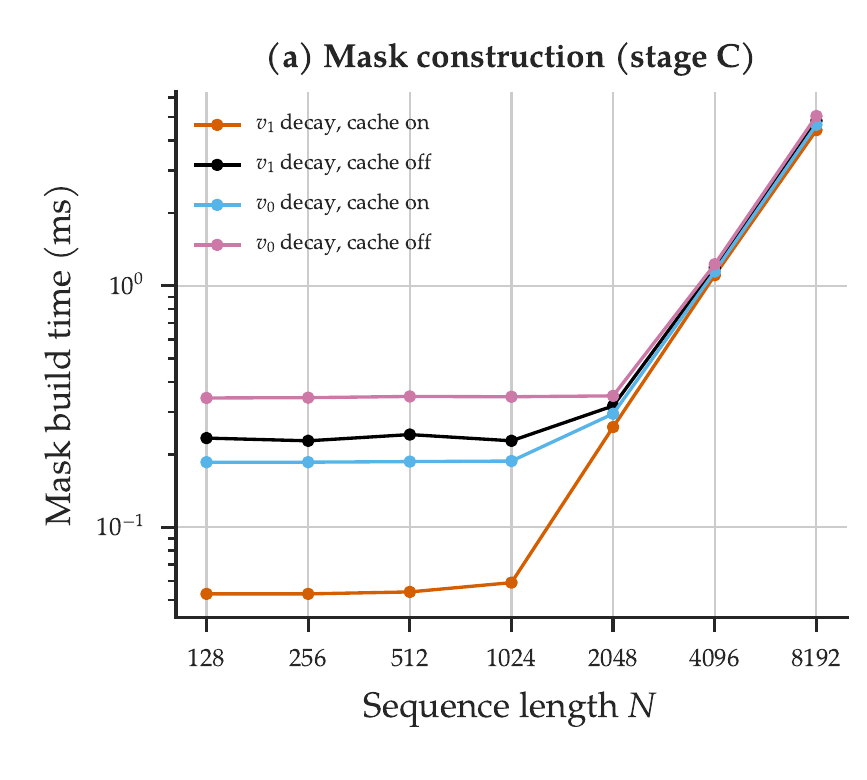
\includegraphics[height=0.56\textheight,keepaspectratio]{mask_construction_panel.png}
    \end{column}
    \begin{column}{0.42\textwidth}
      \centering
      \begin{tikzpicture}[
        card/.style={draw=talkgray!40, fill=talklight, rounded corners=1.5mm,
          text width=38mm, align=center, inner sep=2.2mm, font=\small,
          text=talkgray},
      ]
        \node[card] (one) at (0,0) {%
          {\fontsize{4.5mm}{5.4mm}\selectfont\textcolor{tudblue}{\textbf{4.41 ms}}}\par
          \vspace{1mm}
          {\scriptsize construction at $N{=}8192$}\par
          {\scriptsize 14$\times$ the kernel call}%
        };
        \node[card, below=3mm of one] (two) {%
          {\fontsize{4.5mm}{5.4mm}\selectfont\textcolor{tudblue}{\textbf{1032 MB}}}\par
          \vspace{1mm}
          {\scriptsize bool mask materialization}\par
          {\scriptsize 1.97 ms at $N{=}8192$}%
        };
      \end{tikzpicture}
    \end{column}
  \end{columns}
\end{frame}

% ----------------------------------------------------------------------
% Frame 10 -- cache versus SparseMask.
% (a) Why: the mask can be retained without paying the dense-mask cost.
% (b) Tried: CachedDistAttention distance cache; SparseMask K=16 at B=64.
% (c) Novel: semantics-preserving distance cache; production-batch
%     sparse-mask comparison.
% (d) Interpretation: SparseMask is the practical mask-capable choice;
%     CachedDistAttention is the dense reference. Threat: K=16 only.
% ----------------------------------------------------------------------
\begin{frame}
  \talktitle{If you keep the cutoff, use SparseMask}
  \centering
  \small
  \renewcommand{\arraystretch}{1.35}
  \begin{tabular}{@{}rrrr@{}}
    \toprule
    $N$ & CachedDistAttention (ms) & SparseMask $K{=}16$ (ms) & Speedup\\
    \midrule
    512 & 1.407 & 0.615 & 2.3$\times$\\
    4096 & 85.327 & 21.938 & 3.9$\times$\\
    \bottomrule
  \end{tabular}
  \vspace{5mm}

  {\footnotesize CachedDistAttention caches distances once: 1.26--1.76$\times$ over per-layer recomputation, with identical semantics.\par}
\end{frame}

% ----------------------------------------------------------------------
% Frame 11 -- cutoff ablation.
% (a) Why: the cutoff is often treated as a pure compute knob; test whether
%     removing it is accuracy-neutral.
% (b) Tried: 6-fold leave-one-condition-out, DenseFlash versus
%     CachedDistAttention, 2 seeds.
% (c) Novel: to our knowledge, the first Trackastra cutoff ablation.
% (d) Interpretation: removing the cutoff is not accuracy-neutral; the
%     effect is one-signed but small relative to cross-condition spread.
%     Threat: 2 seeds; no significance test.
% ----------------------------------------------------------------------
\begin{frame}
  \talktitle{Removing the cutoff is not accuracy-neutral}
  \centering
  \small
  \renewcommand{\arraystretch}{1.35}
  \begin{tabular}{@{}p{58mm}p{72mm}@{}}
    \toprule
    \textbf{Result} & \textbf{Value}\\
    \midrule
    Worse fold--seed cells & 12/12 (6 folds $\times$ 2 seeds)\\
    Pooled AOGM penalty & $+47.5$ [32.1, 62.0]\\
    Cutoff occupancy & 42.7\% mean; 23.2\% median\\
    Design & 6-fold leave-one-condition-out; paired\\
    Caveat & 2 seeds; no significance test\\
    \bottomrule
  \end{tabular}
  \vspace{4mm}

  {\footnotesize DenseFlash (cutoff removed) versus CachedDistAttention (cutoff retained).\par}
\end{frame}

% ----------------------------------------------------------------------
% Frame 12 -- equivalence.
% (a) Why: SparseMask can inherit SparseGather's accuracy only if the two
%     implementations agree.
% (b) Tried: 18 configurations, N<=512, K in {4,16}, 3 seeds, fp16.
% (c) Novel: equivalence enabling accuracy transfer without retraining.
% (d) Interpretation: finite numerical agreement, not a proof; valid at the
%     tested configurations. Threat: N<=512.
% ----------------------------------------------------------------------
\begin{frame}
  \talktitle{SparseMask inherits SparseGather accuracy}
  \centering
  \begin{tikzpicture}[
    x=1mm, y=1mm,
    card/.style={draw=talkgray!40, fill=talklight, rounded corners=1.5mm,
      text width=124mm, align=center, inner sep=3mm, minimum height=14mm,
      font=\small, text=talkgray},
  ]
    \node[card, anchor=north] at (72,0)
      {18 configurations; $N{\leq}512$; $K{\in}\{4,16\}$; 3 seeds; fp16};
    \node[card, anchor=north] at (72,-18)
      {Forward $<5\times10^{-4}$; backward $<8\times10^{-4}$};
    \node[card, anchor=north] at (72,-36)
      {$\sim$2 GPU-min versus 600+ for a full training run};
  \end{tikzpicture}
  \vspace{2mm}

  {\footnotesize Finite numerical agreement, not a proof; it licenses accuracy transfer at the tested configurations.\par}
\end{frame}

% ----------------------------------------------------------------------
% Frame 13 -- token reordering.
% (a) Why: the proposal asked whether memory-locality reordering adds gains.
% (b) Tried: SparseGather with spatial token sort on real centroids and
%     random data, L=12, fp16.
% (c) Novel: negative result on real vanvliet centroids.
% (d) Interpretation: negligible gain; discarded. Threat: local measurement.
% ----------------------------------------------------------------------
\begin{frame}
  \talktitle{Token reordering does not help}
  \centering
  \small
  \renewcommand{\arraystretch}{1.35}
  \begin{tabular}{@{}lcc@{}}
    \toprule
    Input & Reorder ratio & Verdict\\
    \midrule
    Real vanvliet centroids\scite{wu2024point} & 0.992--1.023$\times$ & discarded\\
    Random coordinates & 0.97--1.03$\times$ & discarded\\
    \bottomrule
  \end{tabular}
  \vspace{4mm}

  {\footnotesize Proposal item; $L{=}12$; fp16; local measurement.}
\end{frame}

% ----------------------------------------------------------------------
% Frame 14 -- Amdahl and the normalization chain.
% (a) Why: kernel speedup matters only if attention is a large step share.
% (b) Tried: phase decomposition, identity ablation, Amdahl; production loop
%     on five H100 nodes.
% (c) Novel: end-to-end bound with measured shares and the B=1/B=64
%     qualification.
% (d) Interpretation: attention is ~10%; the norm chain is 38.7% and
%     host-side; the measured difference is 2.9% within +/-6%.
%     Threat: per-epoch spread cannot resolve 1.044 vs 1.08.
% ----------------------------------------------------------------------
\begin{frame}
  \talktitle{Attention is not the training bottleneck}
  \centering
  \begin{columns}[c]
    \begin{column}{0.46\textwidth}
      \centering
      {\small\textbf{Step wall}}\par\vspace{1.5mm}
      {\footnotesize
      \renewcommand{\arraystretch}{1.25}
      \begin{tabular}{@{}lr@{}}
        \toprule
        Phase & Share\\
        \midrule
        norm chain & 38.7\%\\
        attention & 10.05\%\\
        other & 51.25\%\\
        \bottomrule
      \end{tabular}}
    \end{column}
    \begin{column}{0.46\textwidth}
      \centering
      {\small\textbf{Amdahl}}\par\vspace{1.5mm}
      {\footnotesize
      \renewcommand{\arraystretch}{1.25}
      \begin{tabular}{@{}lr@{}}
        \toprule
        Assumption & Prediction\\
        \midrule
        $s=0.098$, $k=1.75$ & 1.044\\
        $B{=}64$, $k=6.45$ & $\approx$1.08\\
        measured & 2.9\%, $\pm$6\%\\
        \bottomrule
      \end{tabular}}
    \end{column}
  \end{columns}
  \vspace{3mm}

  {\footnotesize The norm chain is host-side: 240 device synchronizations per step; its GPU kernels are 1.6--2.1\%. Dense baseline (\texttt{knn\_neighbors}$=-1$); the $B{=}1$ $k$ is conservative.\par}
\end{frame}

% ----------------------------------------------------------------------
% Frame 15 -- NSA rejection.
% (a) Why: a sparse-attention candidate was benchmarked and must be resolved.
% (b) Tried: NSA across the measured N grid at B=64.
% (c) Novel: measured rejection at cell-tracking sequence lengths.
% (d) Interpretation: fixed compression and block-selection overhead
%     dominates at small N, not the encoder-decoder architecture.
% ----------------------------------------------------------------------
\begin{frame}
  \talktitle{NSA is rejected at these $N$}
  \centering
  \small
  \renewcommand{\arraystretch}{1.35}
  \begin{tabular}{@{}lr@{}}
    \toprule
    $N$ range & NSA / CachedDistAttention\\
    \midrule
    128--1024 & 11.7$\times$\\
    2048 & 8.5$\times$\\
    4096 & 2.2$\times$\\
    8192 & 1.15$\times$\\
    \bottomrule
  \end{tabular}
  \vspace{4mm}

  {\footnotesize Fixed compression and block-selection overhead dominates at small $N$, not the encoder-decoder architecture.\par}
\end{frame}

% ======================================================================
% 20-ssl.tex -- SPEC 0055, frames 16-23.
%
% §4.2 SSL association pretraining. Eight frames: divider; pretext;
% protocol; result; root cause; coordinate solvability; the frozen DynaCLR
% pivot; status and open branches. No SSL or contrastive tutorial.
% ======================================================================

% ----------------------------------------------------------------------
% Frame 16 -- divider.
% ----------------------------------------------------------------------
\talksectiondivider{\S4.2: Can warps manufacture association labels?}{One question: can a warp supply the label for free?}

% ----------------------------------------------------------------------
% Frame 17 -- why the pretext is not just another augmentation.
% (a) Why: separate the pretext from Trackastra's augmentation stack; the
%     claim is about the supervision source, not the warp type.
% (b) Tried: one frame, warp T, synthetic next frame, labels i -> T(i).
% (c) Novel: annotation-free association-label construction for the
%     low-label regime.
% (d) Interpretation: legitimate SSL idea; target is low-label. Threat: the
%     synthetic pair is not real motion.
% ----------------------------------------------------------------------
\begin{frame}
  \talktitle{Why the warp pretext is not just another augmentation}
  \begin{center}
  \begin{tikzpicture}[
    card/.style={draw=talkblue, fill=talkblue!6, rounded corners=2pt,
      text width=0.86\linewidth, align=center, inner sep=5pt, font=\small}
  ]
    \node[card] (cardone) {Trackastra augmentations perturb annotated windows};
    \node[card, below=4mm of cardone] (cardtwo) {Warp derives $i\to T(i)$\scite{wang2019learning,jabri2020spacetime}};
    \node[card, below=4mm of cardtwo] (cardthree) {No tracking annotations; targets the low-label regime};
  \end{tikzpicture}
  \end{center}
\end{frame}

% ----------------------------------------------------------------------
% Frame 18 -- the protocol.
% (a) Why: test the pretext under a pre-registered low-label rule, not post
%     hoc.
% (b) Tried: pretrain on trpL unlabeled frames (evaluation frames excluded),
%     fine-tune on five labeled pairs, random init and compute-matched
%     control, pre-registered success rule.
% (c) Novel: controlled low-label pilot with a compute-matched control and a
%     held-out condition.
% (d) Interpretation: if the rule fails, report failure; no protocol tweaks.
%     Threat: prototype scale.
% ----------------------------------------------------------------------
\begin{frame}
  \talktitle{What we tried: \texttt{trpL} held out, 5 labeled pairs, compute-matched control}
  \vfill
  \begin{center}
  \begin{tikzpicture}[
    card/.style={draw=talkblue, fill=talkblue!6, rounded corners=2pt,
      text width=0.40\linewidth, align=center, inner sep=5pt, font=\small}
  ]
    \node[card] (cardone) {\texttt{trpL} held out};
    \node[card, right=4mm of cardone] (cardtwo) {5 labeled pairs};
    \node[card, below=4mm of cardone] (cardthree) {random init + compute-matched control};
    \node[card, below=4mm of cardtwo] (cardfour) {pre-registered success rule, fixed before the run};
  \end{tikzpicture}
  \end{center}
  \vfill
\end{frame}

% ----------------------------------------------------------------------
% Frame 19 -- the result.
% (a) Why: does pretraining transfer to the held-out condition?
% (b) Tried: three arms, validation balanced accuracy.
% (c) Novel: the compute-matched control isolates the pretext from extra
%     compute.
% (d) Interpretation: all three arms 0.500; the rule was not met. Threat:
%     balanced accuracy at chance can hide calibration differences.
% ----------------------------------------------------------------------
\begin{frame}
  \talktitle{Result: all three arms 0.500}
  \begin{center}
  \small
  \begin{tabular}{lc}
    \toprule
    Arm & Validation balanced accuracy\\
    \midrule
    Random init & 0.500\\
    Warp pretext & 0.500\\
    Matched control & 0.500\\
    \bottomrule
  \end{tabular}
  \end{center}
  \vspace{4mm}

  \begin{center}
  {\footnotesize Chance is 0.500; the pre-registered success rule was not met.}
  \end{center}
\end{frame}

% ----------------------------------------------------------------------
% Frame 20 -- root cause.
% (a) Why: a null result is only useful with a root cause.
% (b) Tried: loss and entropy analysis, pool dependence, input audit,
%     true-identity accuracy.
% (c) Novel: root-cause evidence for objective-level collapse, not an
%     implementation bug.
% (d) Interpretation: loss 0.161 at the entropy floor; the same recipe
%     learns on another pool; input audit rules out an artifact. Threat:
%     one prototype configuration.
% ----------------------------------------------------------------------
\begin{frame}
  \talktitle{Why it collapsed: $\sim 1/N$ positives and an all-negative optimum}
  \begin{center}
  \begin{tikzpicture}[
    card/.style={draw=talkblue, fill=talkblue!6, rounded corners=2pt,
      text width=0.86\linewidth, align=center, inner sep=5pt, font=\small}
  ]
    \node[card] (cardone) {$\sim 1/N$ positives in the $N{\times}N$ BCE};
    \node[card, below=4mm of cardone] (cardtwo) {all-negative is the analytic optimum};
    \node[card, below=4mm of cardtwo] (cardthree) {loss 0.161 at the entropy floor; control pool 0.10 vs 0.188 floor};
  \end{tikzpicture}
  \end{center}
  \vspace{2mm}

  \begin{center}
  {\footnotesize Input audit: targets match the true correspondence; view-2 appearance is correctly warped; identical code learns on another pool.}
  \end{center}
\end{frame}

% ----------------------------------------------------------------------
% Frame 21 -- coordinate solvability.
% (a) Why: are the warp labels themselves too easy or positionally solvable?
% (b) Tried: coordinate-only probe on 92 frames, 8 experiments, 15 warp
%     draws per frame, seed 42.
% (c) Novel: quantifies coordinate recoverability of the warp labels.
% (d) Interpretation: a property of the labels, not a verdict on the
%     pretext's training value. Threat: applied configuration only.
% ----------------------------------------------------------------------
\begin{frame}
  \talktitle{Coordinate solvability: 0.982 of warp labels recoverable from coordinates}
  \begin{center}
  \small
  \begin{tabular}{@{}lccc@{}}
    \toprule
    Configuration & ICP & Warp-family & Oracle\\
    \midrule
    Applied: affine $10^\circ$, jitter 4, dropout 0.1 & 0.854 & 0.982 & 0.999\\
    Wider: affine $25^\circ$, jitter 8, dropout 0.1 & 0.629 & 0.900 & 0.933\\
    \addlinespace
    \multicolumn{4}{@{}l}{\footnotesize Random baseline $\approx 0.03$ (all columns)}\\
    \bottomrule
  \end{tabular}
  \end{center}
  \vspace{2mm}

  \begin{center}
  {\footnotesize This is a property of the labels, not a verdict on the pretext's training value.}
  \end{center}
\end{frame}

% ----------------------------------------------------------------------
% Frame 22 -- the pivot.
% (a) Why: after the pretext failure, build a legitimate SSL component
%     within scope.
% (b) Tried: DynaCLR-style NT-Xent ScaledCNN, 1.47M parameters, 128-D,
%     frozen; evaluated under Achard's protocol.
% (c) Novel: small from-scratch encoder versus large frozen foundation
%     models; feature-encoder pretraining, not association-head pretraining.
% (d) Interpretation: the pivot is a feature encoder, not the proposed
%     association-head pretraining. Threat: pairing uses tracking-derived
%     masks.
% ----------------------------------------------------------------------
\begin{frame}
  \talktitle{What we did instead: DynaCLR encoder 1.47M, frozen}
  \begin{center}
  {\small DynaCLR \scite{hirata2025dynacl}; Achard protocol \scite{achard2025thesis}.\par}
  \vspace{2mm}
  \begin{tikzpicture}[
    box/.style={draw=talkblue, fill=talkblue!6, rounded corners=2pt,
      align=center, inner sep=5pt, font=\small, minimum height=9mm},
    arrow/.style={-{Latex[length=2mm]}, thick, draw=talkblue}
  ]
    \node[box] (patches) {Cell patches};
    \node[box, right=8mm of patches] (encoder) {ScaledCNN + BatchNorm};
    \node[box, right=8mm of encoder] (embedding) {128-D embedding};
    \node[font=\scriptsize\color{talkgray}, below=1mm of encoder] {frozen};
    \draw[arrow] (patches) -- (encoder);
    \draw[arrow] (encoder) -- (embedding);
  \end{tikzpicture}
  \end{center}
  \vspace{3mm}

  \begin{center}
  {\footnotesize 1.47M parameters versus SAM2.1's 80.8M.}\par
  \vspace{1mm}
  {\footnotesize This is a feature encoder, not the proposed association-head pretraining.}
  \end{center}
\end{frame}

% ----------------------------------------------------------------------
% Frame 23 -- status and open branches.
% (a) Why: make the decision and the remaining work explicit.
% (b) Tried: one applied configuration; no full-scale run, no family sweep.
% (c) Novel: none claimed.
% (d) Interpretation: deprioritized as a scope decision, not disproven.
% ----------------------------------------------------------------------
\begin{frame}
  \talktitle{Deprioritized, not disproven; two branches remain open}
  \begin{columns}[t]
    \begin{column}{0.46\textwidth}
      \centering
      {\small\textbf{Decision}}\par\vspace{2mm}
      \begin{tikzpicture}[
        card/.style={draw=talkblue, fill=talkblue!6, rounded corners=2pt,
          text width=0.92\linewidth, align=center, inner sep=4pt, font=\small}
      ]
        \node[card] (one) {Deprioritized as a scope decision};
        \node[card, below=3mm of one] (two) {Not a measured rejection};
        \node[card, below=3mm of two] (three) {No full-scale run};
      \end{tikzpicture}
    \end{column}
    \begin{column}{0.46\textwidth}
      \centering
      {\small\textbf{Still open}}\par\vspace{2mm}
      \begin{tikzpicture}[
        card/.style={draw=talkorange, fill=talkorange!6, rounded corners=2pt,
          text width=0.92\linewidth, align=center, inner sep=4pt, font=\small}
      ]
        \node[card] (one) {Distortion families};
        \node[card, below=3mm of one] (two) {Low-label vs full-label sweep};
        \node[card, below=3mm of two] (three) {Only one applied configuration};
      \end{tikzpicture}
    \end{column}
  \end{columns}
\end{frame}

% ======================================================================
% 30-features.tex -- SPEC 0055, frames 24-31.
%
% §4.3/§4.4 feature story: what was actually trained, the KNN probe, the
% frozen-encoder injection result, the feature-dependence ablation, and the
% cosine diagnostic. Expert audience; no k-NN, cross-validation, or
% contrastive-learning tutorial. One claim per frame.
% ======================================================================

% Draw one of the three one-claim cards used on frames 25, 26, 28, and 31.
% The fixed height keeps the three-card rows visually level; the card text
% may wrap to two lines but remains a single claim.
\providecommand{\featureCardTfour}[1]{%
  \fcolorbox{talkteal}{talklight}{%
    \parbox[c][17mm][c]{0.285\textwidth}{\centering\small #1}}%
}

% ----------------------------------------------------------------------
% Frame 24 -- divider.
% ----------------------------------------------------------------------
\talksectiondivider{\S4.3/\S4.4: What was actually trained? What do features add?}{Frozen injection and the feature probe.}

% ----------------------------------------------------------------------
% Frame 25 -- what was actually trained.
% (a) Why: clarify what was trained; end-to-end fine-tuning was left open.
% (b) Tried: frozen DynaCLR encoder + projection head + concat with
%     position/regionprops; association head trained on annotations.
% (c) Novel: Achard's injection protocol applied to a small from-scratch
%     encoder.
% (d) Interpretation: tests feature quality under a trained head, not the
%     proposed fine-tuning comparison. Threat: not end-to-end; crop
%     semantics differ.
% ----------------------------------------------------------------------
\begin{frame}
  \talktitle{What was actually trained: frozen injection, not end-to-end fine-tuning}
  \vspace{4mm}
  \centering
  \featureCardTfour{\textcolor{talkorange}{End-to-end fine-tune: left open}}\hfill
  \featureCardTfour{Frozen DynaCLR + projection head}\hfill
  \featureCardTfour{Association head trained on annotations}\par
  \vspace{6mm}
\end{frame}

% ----------------------------------------------------------------------
% Frame 26 -- probe design.
% (a) Why: isolate feature information independently of end-to-end training.
% (b) Tried: for each anchor, K=8 nearest cells by centroid; shared MLP
%     scores each pair; three probe seeds; frame-CV and LOCO.
% (c) Novel: coordinates-only candidate construction; the feature cannot
%     select its own shortlist.
% (d) Interpretation: measures re-identification among plausible
%     neighbours, not tracking. Threat: candidate set is geometry-defined.
% ----------------------------------------------------------------------
\begin{frame}
  \talktitle{KNN probe: K=8 covers 99.3\%, candidates by centroid, shared MLP}
  \vspace{4mm}
  \centering
  \featureCardTfour{\textcolor{talkteal}{\textbf{K=8}} covers 99.3\%}\hfill
  \featureCardTfour{Candidates by centroid; feature never selects}\hfill
  \featureCardTfour{Shared MLP, 3 seeds, frame-CV + LOCO}\par
  \vspace{4mm}

  \begin{center}
  {\footnotesize The feature cannot choose its own shortlist.}
  \end{center}
\end{frame}

% ----------------------------------------------------------------------
% Frame 27 -- probe result.
% (a) Why: which signal carries association: position/geometry or learned
%     features?
% (b) Tried: eight feature rows, K=8 MLP, frame-CV/LOCO, nearest-centroid
%     K=1 baseline.
% (c) Novel: LOCO comparison with coordinates-only candidates.
% (d) Interpretation: position and geometry dominate; the DynaCLR margin
%     over nearest-centroid is 0.015. Threat: within-experiment probe.
% ----------------------------------------------------------------------
\begin{frame}
  \talktitle{Position and geometry dominate: DynaCLR 0.826, nearest-centroid 0.811}
  \vspace{1mm}
  \begin{center}
  \scriptsize
  \setlength{\tabcolsep}{7pt}
  \begin{tabular}{lrr}
    \toprule
    \multicolumn{3}{c}{K=8 candidates, 3 probe seeds}\\
    \midrule
    Feature & Frame-CV & LOCO\\
    \midrule
    Regionprops 13D & 0.8694 & 0.8183\\
    Hu 20D & 0.8679 & 0.8023\\
    \textcolor{talkteal}{\textbf{DynaCLR}}\scite{hirata2025dynacl} & \textcolor{talkteal}{\textbf{0.8527}} & \textcolor{talkteal}{\textbf{0.8259}}\\
    Regionprops 7D & 0.8422 & 0.7915\\
    position-only & 0.8127 & 0.7887\\
    SAM2.1\scite{ravi2024sam2} & 0.7354 & 0.7256\\
    DINOv2\scite{oquab2024dinov2} & 0.6782 & 0.6433\\
    NT-Xent & 0.5778 & 0.5634\\
    \midrule
    nearest-centroid & 0.812 & 0.811\\
    \bottomrule
  \end{tabular}
  \end{center}
\end{frame}

% ----------------------------------------------------------------------
% Frame 28 -- what the probe means.
% (a) Why: interpret the ranking without overclaiming.
% (b) Tried: compare feature rows and baselines; frame-CV and LOCO.
% (c) Novel: a large foundation model is not automatically better here.
% (d) Interpretation: features add little over explicit geometry; the
%     ranking is not a tracking verdict. Threat: one checkpoint per feature.
% ----------------------------------------------------------------------
\begin{frame}
  \talktitle{What the probe means: features add little over geometry}
  \vspace{4mm}
  \centering
  \featureCardTfour{Features add little over geometry}\hfill
  \featureCardTfour{SAM2.1 mid-pack}\hfill
  \featureCardTfour{\textcolor{talkred}{NT-Xent 0.563}}\par
  \vspace{6mm}
\end{frame}

% ----------------------------------------------------------------------
% Frame 29 -- injection protocol.
% (a) Why: need a controlled integration to test features in the tracker.
% (b) Tried: projection head + concat during token construction; encoder
%     frozen; head trained on annotations.
% (c) Novel: the reference protocol applied to the 1.47M encoder.
% (d) Interpretation: changes token construction only; no encoder
%     fine-tuning. Threat: crop semantics and protocol mismatch.
% ----------------------------------------------------------------------
\begin{frame}
  \talktitle{Injection protocol: projection head + concat; encoder frozen}
  \vspace{3mm}
  \centering
  \begin{tikzpicture}[
    box/.style={draw=talkteal, fill=talklight, rounded corners=1.2mm,
                text width=30mm, minimum height=11mm, align=center,
                inner sep=1.5mm, font=\small},
    arr/.style={-{Stealth[length=2.4mm]}, thick, draw=talkgray},
    lab/.style={font=\scriptsize, text=talkgray, text width=32mm,
                align=center}
  ]
    \node[box] (features) {Learned features};
    \node[box, right=10mm of features] (projection) {projection head\scite{achard2025thesis}};
    \node[circle, draw=talkteal, fill=talklight, inner sep=1.6mm,
          right=10mm of projection] (concat) {$\oplus$};
    \node[box, right=10mm of concat] (token) {transformer token};
    \node[box, above=8mm of concat] (position) {Fourier PE};
    \node[box, below=8mm of concat] (geometry) {regionprops};
    \draw[arr] (features) -- (projection);
    \draw[arr] (projection) -- (concat);
    \draw[arr] (position) -- (concat);
    \draw[arr] (geometry) -- (concat);
    \draw[arr] (concat) -- (token);
    \node[lab, below=1mm of projection] {linear + LayerNorm};
  \end{tikzpicture}
  \vspace{3mm}
\end{frame}

% ----------------------------------------------------------------------
% Frame 30 -- Bacteria and DeepCell in one figure.
% (a) Why: does the small encoder help in-domain and transfer?
% (b) Tried: frozen DynaCLR + Achard injection, 3 seeds; Bacteria and
%     DeepCell with the 91/27 head split.
% (c) Novel: 1.47M from-scratch encoder versus SAM2.1 and other frozen
%     features.
% (d) Interpretation: competitive, not state of the art; DeepCell parity is not a win;
%     the remaining gap to Original Trackastra is detection.
% ----------------------------------------------------------------------
\begin{frame}
  \talktitle{Small encoder is competitive, not state of the art}
  \vspace{1mm}
  \centering
  {\small Reference protocol \scite{achard2025thesis}; SAM2.1 \scite{ravi2024sam2}; Bacteria \scite{vanvliet2018}; DeepCell \scite{schwartz2023}.\par}
  \vspace{1mm}
  \includegraphics[height=0.54\textheight,keepaspectratio]{18_feature_injection_comparison.pdf}\par
  \vspace{1mm}
  {\footnotesize Bacteria 8.81 vs SAM2.1 7.00; DeepCell 19.35 vs 19.93; Original Trackastra 11.9 (greedy). The remaining DeepCell gap is detection.\par}
\end{frame}

% ----------------------------------------------------------------------
% Frame 31 -- interpretation.
% (a) Why: synthesize §4.4 without overclaiming.
% (b) Tried: combine probe + injection + dependence + cosine results.
% (c) Novel: small encoder competitive; position is the signal.
% (d) Interpretation: 1.47M competitive; position/geometry dominate; no
%     state-of-the-art claim and no low-label gain. Threat: one encoder; one crop protocol.
% ----------------------------------------------------------------------
\begin{frame}
  \talktitle{\S4.4 interpretation: small encoder competitive; position is the signal}
  \vspace{4mm}
  \centering
  \featureCardTfour{\textcolor{talkteal}{\textbf{1.47M}} competitive}\hfill
  \featureCardTfour{Position is the signal}\hfill
  \featureCardTfour{\textcolor{talkred}{Not state of the art}}\par
  \vspace{6mm}
\end{frame}

% ======================================================================
% 40-synthesis.tex -- SPEC 0055, frames 32-36.
%
% Insight-first synthesis. Five frames: what changed and how it was caught;
% what was not done and why; recommendations; next steps; what the results
% do not license. The duplicate exploration table and the novelty inventory
% from SPEC 0054 are removed. Frame 37 (thank you) is in 50-close.tex.
% ======================================================================

% ----------------------------------------------------------------------
% Frame 32 -- what changed, and how it was caught.
% Process frame: each row names a changed belief and the measurement that
% changed it. No new claims; every value is from the report.
% ----------------------------------------------------------------------
\begin{frame}
  \talktitle{What changed, and how we caught it}
  \centering
  \hyphenpenalty=10000
  \exhyphenpenalty=10000
  \scriptsize
  \renewcommand{\arraystretch}{1.30}
  \setlength{\tabcolsep}{1.8mm}
  \begin{tabular}{@{}p{53mm}>{\raggedright\arraybackslash}p{83mm}@{}}
    \toprule
    \textbf{Changed belief} & \textbf{How we caught it}\\
    \midrule
    The mask cost is not a kernel-package cost. &
    Forced-backend arms and per-row kernel names; masked SDPA reaches fused cuDNN.\\
    The cutoff is not only a compute knob. &
    Paired 6-fold leave-one-condition-out ablation: 12/12 fold--seed cells worse.\\
    The warp pretext does not transfer at prototype scale. &
    Pre-registered low-label pilot failed; loss at the entropy floor; input audit ruled out a bug.\\
    Learned features are not the main association signal. &
    Coordinates-only candidates; ScaledCNN LOCO 0.826 vs nearest-centroid 0.811.\\
    The delivered SSL component is a feature encoder. &
    Frozen ScaledCNN injection; the proposed association-head pretraining was not delivered.\\
    \bottomrule
  \end{tabular}
\end{frame}

% ----------------------------------------------------------------------
% Frame 33 -- what was not done and why.
% Process frame: explicit negative/omitted work. Keeps the statuses
% distinct and pre-empts the obvious expert questions.
% ----------------------------------------------------------------------
\begin{frame}
  \talktitle{What we did not do, and why}
  \centering
  \hyphenpenalty=10000
  \exhyphenpenalty=10000
  \scriptsize
  \renewcommand{\arraystretch}{1.30}
  \setlength{\tabcolsep}{1.8mm}
  \begin{tabular}{@{}p{53mm}>{\raggedright\arraybackslash}p{83mm}@{}}
    \toprule
    \textbf{Not done} & \textbf{Why}\\
    \midrule
    Full Trackastra port &
    Optional in the proposal; not attempted. The 18-configuration test checks SparseGather/SparseMask equivalence, not a port.\\
    Token reordering &
    0.992--1.023$\times$ on real centroids; discarded.\\
    NSA &
    11.7$\times$ slower than CachedDistAttention at $N{=}128$--$1024$; fixed overhead dominates at small $N$.\\
    Distortion-family and low-label sweep &
    Open beyond the prototype; only affine $10^\circ$ + jitter 4 + dropout 0.1 was piloted.\\
    \bottomrule
  \end{tabular}
\end{frame}

% ----------------------------------------------------------------------
% Frame 34 -- recommendations.
% Each recommendation is tied to a measured value. "Do not optimize
% attention first" is a priority statement, not a claim that attention
% never matters.
% ----------------------------------------------------------------------
\begin{frame}
  \talktitle{Recommendations for the Trackastra team}
  \centering
  \hyphenpenalty=10000
  \exhyphenpenalty=10000
  \scriptsize
  \renewcommand{\arraystretch}{1.30}
  \setlength{\tabcolsep}{1.8mm}
  \begin{tabular}{@{}p{46mm}>{\raggedright\arraybackslash}p{90mm}@{}}
    \toprule
    \textbf{Recommendation} & \textbf{Evidence}\\
    \midrule
    \textbf{Keep the cutoff} &
    Removing it is worse in 12/12 fold--seed cells; pooled $+47.5$ AOGM [32.1, 62.0].\\
    \textbf{Set $K{=}16$} &
    In-sample 201.8 vs 200.8 AOGM; held-out \texttt{trpL} 51.0 vs 43.3. $K{=}32$ is the accuracy-first alternative.\\
    \textbf{Use SparseMask} &
    2.3$\times$ at $N{=}512$ and 3.9$\times$ at $N{=}4096$ versus CachedDistAttention.\\
    \textbf{Do not optimize attention first} &
    10.05\% of the step; Amdahl 1.044 versus 2.9\% measured.\\
    \textbf{Normalize the chain} &
    38.7\% of the step and 240 synchronizations per step: the real target.\\
    \bottomrule
  \end{tabular}
  \vspace{3mm}

  {\footnotesize The cutoff ablation is, to our knowledge, the first for Trackastra.}
\end{frame}

% ----------------------------------------------------------------------
% Frame 35 -- next steps.
% Ordered by expected value: HOCT changes the representation most directly;
% end-to-end training tests the open §4.3 question; the linker ablation
% removes an attribution confound; multi-seed/HP widens every remaining
% claim but changes no mechanism by itself.
% ----------------------------------------------------------------------
\begin{frame}
  \talktitle{What I would do next}
  \centering
  \hyphenpenalty=10000
  \exhyphenpenalty=10000
  \footnotesize
  \renewcommand{\arraystretch}{1.35}
  \setlength{\tabcolsep}{1.8mm}
  \begin{tabular}{@{}p{5mm}p{34mm}p{94mm}@{}}
    \toprule
    \textbf{\#} & \textbf{Next step} & {\raggedright\textbf{What changes}}\\
    \midrule
    1 & \textbf{HOCT edge-centric\scite{bragantini2026hoct}} &
    {\raggedright Replace node-level token features with edge-centric HOCT edge tokens.}\\
    2 & \textbf{End-to-end encoder} &
    {\raggedright Unfreeze and fine-tune the encoder; the current protocol is frozen injection.}\\
    3 & \textbf{Linker ablation} &
    {\raggedright Separate association-head quality from the linker effect on the metric.}\\
    4 & \textbf{Multi-seed / HP} &
    {\raggedright Widen beyond the two CV seeds and add a hyperparameter search before treating small gaps as stable.}\\
    \bottomrule
  \end{tabular}
\end{frame}

% ----------------------------------------------------------------------
% Frame 36 -- what the results do not license.
% Combines the SPEC 0054 limitations and non-claims into one frame. The
% values stay visible so an audience member can challenge a row directly.
% ----------------------------------------------------------------------
\begin{frame}
  \talktitle{What these results do not license}
  \centering
  \hyphenpenalty=10000
  \exhyphenpenalty=10000
  \scriptsize
  \renewcommand{\arraystretch}{1.25}
  \setlength{\tabcolsep}{1.8mm}
  \begin{tabular}{@{}p{42mm}>{\raggedright\arraybackslash}p{94mm}@{}}
    \toprule
    \textbf{Not licensed} & \textbf{Why}\\
    \midrule
    \textbf{No state-of-the-art claim} &
    Bacteria 8.81 vs SAM2.1 7.00; DeepCell 19.35 vs 19.93; still behind Original Trackastra 11.9.\\
    \textbf{No large-$N$ accuracy} &
    The operator benchmark reaches $N{=}32768$; tracking accuracy at thousands of cells is untested.\\
    \textbf{No association-head pretraining} &
    The delivered component is a frozen ScaledCNN encoder; the warp pretext was deprioritized.\\
    \textbf{No low-label gain} &
    Pilot arms all 0.500; the pre-registered success rule was not met.\\
    \textbf{No significance test} &
    Two seeds, 6-fold CV; the 12 fold--seed cells share training data.\\
    \bottomrule
  \end{tabular}
  \vspace{3mm}

  {\footnotesize One encoder, one crop protocol; distortion families were not swept.}
\end{frame}

% ======================================================================
% 50-close.tex -- SPEC 0055, frame 37.
%
% Closing frame. The TUD theme has no dedicated closing macro, so this
% reuses the title-page palette (tudbg/tudwhite) and title face from
% 00-opening.tex/beamerthemeTUD.sty without adding any new theme asset.
% The frame is plain: a closing page carries no footer chrome.
% ======================================================================

\begin{frame}[plain]
  \begin{tikzpicture}[remember picture,overlay]
    \fill[tudbg] (current page.south west) rectangle (current page.north east);
    \node at (current page.center) {%
      \TudTitleFont\fontsize{7.3333mm}{8mm}\selectfont
      \textcolor{tudwhite}{Thank you}};
    \node[anchor=north] at ([yshift=-14mm]current page.center) {%
      \fontsize{3.3333mm}{4mm}\selectfont
      \textcolor{tudwhite}{Questions \& discussion}};
  \end{tikzpicture}
\end{frame}

% ======================================================================
% 90-backup.tex -- SPEC 0055, backup slides B1-B10 (untimed Q&A material).
%
% Every number and image here is copied from a report table/section named
% in SPEC 0055; no talk-only figure and no stale 0053 deck asset is used.
% The frames are intentionally denser than the main deck but remain
% single-screen readable at Q&A distance.
% ======================================================================

% ----------------------------------------------------------------------
% B1 -- full speed detail.
% Source: report-shorten/figs/01_speed_vs_n_h100_detail.pdf. The report
% memory figure is deliberately omitted here: its "A100/H100 80 GB"
% annotation collides with the SparseMask projection, so B2 stays the
% full-width mask view instead.
% ----------------------------------------------------------------------
\begin{frame}
  \talktitle{Full speed detail}
  \centering
  \includegraphics[width=\textwidth,height=0.58\textheight,keepaspectratio]{01_speed_vs_n_h100_detail.pdf}


\end{frame}

% ----------------------------------------------------------------------
% B2 -- full three-panel mask decomposition.
% The main deck uses only panel (a); this is the uncropped report figure.
% It stays full-width so the wide three-panel figure remains readable.
% ----------------------------------------------------------------------
\begin{frame}
  \talktitle{Full mask decomposition}
  \centering
  \includegraphics[width=\textwidth,height=0.58\textheight,keepaspectratio]{20_mask_decomposition.pdf}


\end{frame}

% ----------------------------------------------------------------------
% B3 -- cutoff occupancy.
% Source: report-shorten/figs/masked_fraction.png and sec:app_masked_fraction.
% ----------------------------------------------------------------------
\begin{frame}
  \talktitle{Cutoff occupancy}
  \small
  \renewcommand{\arraystretch}{1.15}
  \setlength{\tabcolsep}{6pt}
  {\raggedright
  \begin{tabular}{@{}lr@{}}
    \toprule
    Condition & Masked fraction \\
    \midrule
    cib & 25.5\% \\
    metA & 38.5\% \\
    pheA & 42.9\% \\
    recA & 50.3\% \\
    rpsM & 54.4\% \\
    trpL & 38.6\% \\
    \midrule
    Mean & 42.7\% \\
    Median & 23.2\% \\
    \bottomrule
  \end{tabular}\par}


\end{frame}

% ----------------------------------------------------------------------
% B4 -- kernel verification and equivalence.
% Sources: tab:attn_names (dispatch/kernel names), sec:equiv_val
% (18 configurations and the forward/backward tolerances).
% ----------------------------------------------------------------------
\begin{frame}
  \talktitle{Kernel verification and equivalence}
  \centering
  \scriptsize
  \renewcommand{\arraystretch}{1.0}
  \setlength{\tabcolsep}{1.6mm}
  \begin{tabular}{@{}p{40mm}p{55mm}p{40mm}@{}}
    \toprule
    \textbf{Architecture} & \textbf{Benchmark key and setting} & \textbf{Verified kernel} \\
    \midrule
    RelativePositionalAttention & \texttt{dense\_masked} (cache off) & cuDNN \\
    CachedDistAttention & \texttt{dense\_masked} (cache on), \texttt{knn}$=-1$ & cuDNN \\
    DenseFlash & \texttt{dense\_flash}, \texttt{knn}$=-2$ & flash \\
    SparseGather & \texttt{gather\_matmul}, \texttt{knn}$>0$ & flash/cuBLAS \\
    SparseMask & \texttt{mask\_knn}, \texttt{knn}$>0$ & cuDNN \\
    \bottomrule
  \end{tabular}
  \vspace{3mm}

  {\footnotesize Measured on H100 / torch 2.14 at $d_{\text{head}}{=}64$; Trackastra's real $d_{\text{head}}{=}40$ is also served by cuDNN.}


\end{frame}

% ----------------------------------------------------------------------
% B5 -- K-sweep and the K=16 recommendation.
% Sources: knn_sweep_metrics_bootstrap.pdf and tab:knn_sweep_multi.
% Values are three-seed means: in-sample AOGM / held-out trpL AOGM.
% ----------------------------------------------------------------------
\begin{frame}
  \talktitle{K-sweep and K=16}
  \centering
  \begin{minipage}{0.61\textwidth}
    \centering
    \includegraphics[width=\linewidth,height=0.58\textheight,keepaspectratio]{knn_sweep_metrics_bootstrap.pdf}
  \end{minipage}\hfill
  \begin{minipage}{0.35\textwidth}
    \centering
    \scriptsize
    \renewcommand{\arraystretch}{1.25}
    \setlength{\tabcolsep}{1.2mm}
    \begin{tabular}{@{}lcc@{}}
      \toprule
      \textbf{$K$} & \textbf{In-sample} & \textbf{Held-out} \\
      \midrule
      Dense & 200.8 & 43.3 \\
      16 & 201.8 & 51.0 \\
      8 & 203.0 & 73.0 \\
      32 & 204.9 & 43.9 \\
      \bottomrule
    \end{tabular}


  \end{minipage}
\end{frame}

% ----------------------------------------------------------------------
% B6 -- full probe table.
% Source: tab:edge_probe_knn; same values as main frame 27, with spreads.
% ----------------------------------------------------------------------
\begin{frame}
  \talktitle{Probe table}
  \centering
  \scriptsize
  \renewcommand{\arraystretch}{1.12}
  \setlength{\tabcolsep}{1.4mm}
  \begin{tabular}{@{}p{48mm}ccc@{}}
    \toprule
    \textbf{Feature} & \textbf{Frame-CV top-1} & \textbf{LOCO top-1} &
    \textbf{LOCO F1} \\
    \midrule
    ScaledCNN (DynaCLR recipe) & $0.8527 \pm 0.0044$ & $0.8259 \pm 0.0054$ &
    $0.8279 \pm 0.0053$ \\
    Regionprops 13D & $0.8694 \pm 0.0008$ & $0.8183 \pm 0.0035$ &
    $0.8174 \pm 0.0024$ \\
    Hu 20D & $0.8679 \pm 0.0014$ & $0.8023 \pm 0.0052$ &
    $0.8115 \pm 0.0040$ \\
    Regionprops 7D & $0.8422 \pm 0.0046$ & $0.7915 \pm 0.0020$ &
    $0.7898 \pm 0.0024$ \\
    Position-only & $0.8127 \pm 0.0013$ & $0.7887 \pm 0.0040$ &
    $0.7743 \pm 0.0033$ \\
    SAM2.1-Hiera-B+ (frozen) & $0.7354 \pm 0.0026$ & $0.7256 \pm 0.0044$ &
    $0.7192 \pm 0.0036$ \\
    DINOv2 (frozen) & $0.6782 \pm 0.0042$ & $0.6433 \pm 0.0043$ &
    $0.6520 \pm 0.0031$ \\
    CNN NT-Xent (frozen) & $0.5778 \pm 0.0037$ & $0.5634 \pm 0.0004$ &
    $0.5604 \pm 0.0011$ \\
    \midrule
    Nearest-centroid ($K{=}1$) & 0.812 & 0.811 & n/a \\
    \bottomrule
  \end{tabular}


\end{frame}

% ----------------------------------------------------------------------
% B7 -- full injection table.
% Source: tab:feature_injection. Point estimates are left without a
% spread where the reference publishes none.
% ----------------------------------------------------------------------
\begin{frame}
  \talktitle{Injection table}
  \centering
  \scriptsize
  \renewcommand{\arraystretch}{1.18}
  \setlength{\tabcolsep}{1.6mm}
  \begin{tabular}{@{}p{40mm}p{24mm}p{24mm}p{40mm}@{}}
    \toprule
    \textbf{Method} & \textbf{Bacteria AOGM} & \textbf{DeepCell AOGM} &
    \textbf{Exposure} \\
    \midrule
    General-2D (Trackastra) & 49.58 & 23.04 & in-domain \\
    WRFEAT-DO & $11.25 \pm 3.67$ & $19.31 \pm 0.55$ & in-domain \\
    SAM2.1-Hiera-B+ & $7.00 \pm 2.14$ & $19.93 \pm 1.15$ & zero-shot \\
    CoTracker3 & $20.81 \pm 5.41$ & $18.62 \pm 0.99$ & zero-shot \\
    Original Trackastra (greedy) & 29.0 & 11.9 & in-domain; GT detections \\
    ScaledCNN (DynaCLR recipe, ours) & $8.81 \pm 2.11$ & $19.35 \pm 0.76$ &
    Bacteria in-domain; DeepCell test held out (91/27) \\
    \bottomrule
  \end{tabular}


\end{frame}

% ----------------------------------------------------------------------
% B8 -- pretext and coordinate solvability.
% Sources: tab:app_pretext and sec:pretext.
% ----------------------------------------------------------------------
\begin{frame}
  \talktitle{Pretext and coordinate solvability}
  \centering
  \scriptsize
  \renewcommand{\arraystretch}{1.2}
  \setlength{\tabcolsep}{2mm}
  \begin{minipage}{0.92\textwidth}
    \centering
    \begin{tabular*}{\linewidth}{@{\extracolsep{\fill}}p{52mm}cccc@{}}
      \toprule
      \textbf{Configuration} & \textbf{ICP} & \textbf{Warp-family solver} &
      \textbf{Oracle} & \textbf{Random} \\
      \midrule
      Applied (affine $10^\circ$ + jitter 4 + dropout 0.1) &
      \textbf{0.854} & \textbf{0.982} & \textbf{0.999} & 0.032 \\
      Wider (affine $25^\circ$ + jitter 8 + dropout 0.1) &
      0.629 & 0.900 & 0.933 & 0.031 \\
      \bottomrule
    \end{tabular*}

    \vspace{4mm}
    \begin{tabular*}{\linewidth}{@{\extracolsep{\fill}}p{64mm}p{58mm}@{}}
      \toprule
      \textbf{Collapse audit} & \textbf{Value} \\
      \midrule
      Random init / warp pretext / matched control & 0.500 / 0.500 / 0.500 \\
      Pretext SSL loss & 0.161 (entropy floor of a constant predictor) \\
      Matched control pool loss & 0.10 vs 0.188 floor \\
      \bottomrule
    \end{tabular*}
  \end{minipage}


\end{frame}

% ----------------------------------------------------------------------
% B9 -- epoch/Amdahl and architecture complexity.
% Sources: sec:eval_amdahl and tab:complexity.
% ----------------------------------------------------------------------
\begin{frame}
  \talktitle{Amdahl and complexity}
  \centering
  \begin{minipage}{0.39\textwidth}
    \centering
    \scriptsize
    \renewcommand{\arraystretch}{1.12}
    \setlength{\tabcolsep}{1.4mm}
    \begin{tabular}{@{}p{30mm}r@{}}
      \toprule
      \textbf{Epoch / step share} & \textbf{Value} \\
      \midrule
      Batch phase & 97.7\% \\
      Dataloader & 0.5\% \\
      Validation & 1.1\% \\
      Residual overhead & $\sim$0.7\% \\
      Normalization chain & 38.7\% \\
      Attention & 10.05\% \\
      GPU kernels & $\sim$48\% \\
      Norm GPU kernels & 1.6--2.1\% \\
      \midrule
      Amdahl share $s$ & 0.098 \\
      Predicted, $k\approx1.75$ & 1.044 \\
      Predicted, $B{=}64$ ratio & $\approx$1.08 \\
      Measured per-epoch & 2.9\% \\
      Three-seed CV spread & $\pm$6\% \\
      \bottomrule
    \end{tabular}
  \end{minipage}\hfill
  \begin{minipage}{0.58\textwidth}
    \centering
    \scriptsize
    \renewcommand{\arraystretch}{1.25}
    \setlength{\tabcolsep}{0.8mm}
    \begin{tabular}{@{}p{40mm}ccp{8mm}@{}}
      \toprule
      \textbf{Architecture} & \textbf{Compute} & \textbf{Memory} & \textbf{Loc.} \\
      \midrule
      RelativePositionalAttention & $\mathcal{O}(N^2d)$ & $\mathcal{O}(N^2)$ & yes \\
      CachedDistAttention & $\mathcal{O}(N^2d)$ & $\mathcal{O}(N^2)$ & yes \\
      DenseFlash & $\mathcal{O}(N^2d)$ & $\mathcal{O}(N)$ & no \\
      SparseGather & $\mathcal{O}(Nkd)$ & $\mathcal{O}(Nk)$ & yes \\
      SparseMask & $\mathcal{O}(Nkd)$ & $\mathcal{O}(N^2)$ & yes \\
      \bottomrule
    \end{tabular}


  \end{minipage}
\end{frame}

% ----------------------------------------------------------------------
% B10 -- feature-use and cosine controls.
% Q&A only. The report carries these as one prose sentence. The zero row is
% an out-of-distribution probe, not a no-feature trained baseline. The
% cosine-only value predates the aggregation correction and has no current
% stored artifact. Do not promote to a main-deck claim.
% ----------------------------------------------------------------------
\begin{frame}
  \talktitle{Feature-use and cosine controls (report prose only)}
  \centering
  \begin{minipage}{0.46\textwidth}
    \centering
    {\small\textbf{Feature-use control}}\par\vspace{2mm}
    \scriptsize
    \renewcommand{\arraystretch}{1.2}
    \begin{tabular}{@{}lr@{}}
      \toprule
      Feature condition & Bacteria AOGM\\
      \midrule
      normal & 8.81\\
      shuffled & 9.75\\
      zeroed (out of distribution) & 150.6\\
      \bottomrule
    \end{tabular}
  \end{minipage}\hfill
  \begin{minipage}{0.46\textwidth}
    \centering
    {\small\textbf{Cosine-only protocol}}\par\vspace{2mm}
    \scriptsize
    \renewcommand{\arraystretch}{1.2}
    \begin{tabular}{@{}lr@{}}
      \toprule
      Quantity & Value\\
      \midrule
      AOGM & $\sim$88332\\
      same-cell cosine & 0.987\\
      different-cell cosine & 0.968\\
      \bottomrule
    \end{tabular}
  \end{minipage}
  \vspace{4mm}

  {\footnotesize No matched no-feature trained arm exists. The zero row is an OOD probe, not evidence that features help. The cosine value predates the current aggregation correction and has no current stored artifact. Keep as Q\&A material only.}
\end{frame}

% ----------------------------------------------------------------------
% References -- final backup frame.
% Renders every citation used in the deck; biber reads references.bib.
% ----------------------------------------------------------------------
\begin{frame}[allowframebreaks]
  \talktitle{References}
  \vspace*{6mm}
  \begingroup
  \tiny
  \renewcommand*{\bibfont}{\tiny}
  \setlength{\bibitemsep}{0pt}
  \setlength{\bibhang}{0pt}
  \printbibliography[heading=none]
  \endgroup
\end{frame}


\end{document}
